%https://github.com/milizeus/MFP-flashcards.git
%
\documentclass[a5paper,12pt,ngerman,grid=front %
%,toc % funktioniert nicht in Kombination mit print
,print
]{kartei}
\usepackage{hyperref}
\usepackage[german]{babel}
\usepackage[T1]{fontenc}
\usepackage[latin1]{inputenc}
%\usepackage[utf8x]{inputenc}
\usepackage{amsmath}
\usepackage{amssymb}
\usepackage{graphicx}
\usepackage[version=3]{mhchem}
\usepackage{gensymb}
\usepackage{enumitem} 
\let\oldce\ce
\renewcommand*{\ce}[1]{\begingroup\color{red}\oldce{#1}\endgroup}
%%%%%%%%%%%%%%%%%%%%%%%%%%%%%%%%%%%%%%%%%%%%%%%%%%%%%%%%%%%%%%%%%%%%%%%%%%
%%%%%%%%%%%%%%%%%%%%%%%%%%%%%%%%%%%%%%%%%%%%%%%%%%%%%%%%%%%%%%%%%%%%%%%%%%


\title{Pr�fungsfragen Chemie}
%%%%%%%%%%%%%%%%%%%%%%%%%%%%%%%%%%%%%%%%%%%%%%%%%%%%%%%%%%%%%%%%%%%%%%%%%%


\begin{document}
\setcardpagelayout





	
		%%%%%%%%%%%%%%%%%%%%%%%%%%%%%%%%%%%%%%%%%%%%%%%%%%%%%%%%%%%%%%%%%%%%%%%%%%
%%%%%%%%%%%%%%%%%%%%%%%%%%%%%%%%%%%%%%%%%%%%%%%%%%%%%%%%%%%%%%%%%%%%%%%%%%
\section*{ST"OCHIOMETRIE}
%%%%%%%%%%%%%%%%%%%%%%%%%%%%%%%%%%%%%%%%%%%%%%%%%%%%%%%%%%%%%%%%%%%%%%%%%%
%%%%%%%%%%%%%%%%%%%%%%%%%%%%%%%%%%%%%%%%%%%%%%%%%%%%%%%%%%%%%%%%%%%%%%%%%%



%%%%%%%%%%%%%%%%%%%%%%%%%%%%%%%%%%%%%%%%%%%%%%%%%%%%%%%%%%%%%%%%%%%%%%%%%%%%%%%%
\begin{karte}{
	%%%%%%%%%%%%%%%%%%%%%%%%%%%%%%%%%%%%%%%%%%%%%%%%%%%%%%%%%%%%
	%Frage
	Stellen Sie sich vor, Sie wollen einen Prozess verbessern, in dem aus Eisenerz, das \ce{Fe_{2}O_{3}} enth�lt, Eisen gewonnen wird. Als Testexperiment f�hren sie folgende Reaktion durch: \ce{Fe_{2}O_{3} +3CO -> 2Fe +3CO_{2}}\\
	Schreiben Sie f�r alle Atome die Oxidationszahlen an. \\
	Wenn Sie mit 150 g \ce{Fe_{2}O_{3}} limitierendem Reaktanten beginnen, wie gro� ist die theoretische Ausbeute an \ce{Fe}? \\
	Wie gro� w�re die prozentuale Ausbeute, wenn Ihre tats�chliche Ausbeute an \ce{Fe} 87.9 g w�re?
	%%%%%%%%%%%%%%%%%%%%%%%%%%%%%%%%%%%%%%%%%%%%%%%%%%%%%%%%%%%%
	}
	%%%%%%%%%%%%%%%%%%%%%%%%%%%%%%%%%%%%%%%%%%%%%%%%%%%%%%%%%%%%
	%Antwort
	\begin{itemize}
		\item
			Oxidationszahlen: 
			\ce{Fe2^{3+} O3 ^{2-} +3C ^{2+} O ^{2-} -> 2Fe^{0} + 3C^{4+}O2^{2-}}
		\item
			theoretische Ausbeute:\\ \\
			Mol berechnen, Stoffmenge mit Atomgewicht multiplizieren\\
			theoretische Ausbeute= $x  Mol \cdot x \frac{g}{Mol}$\\ 
			
			$M_{\ce{Fe2O3}}= 2\cdot55,8+3\cdot16= 159,6 g/Mol$ \\
			$M_{\ce{3CO}}=3\cdot(12+16)=84 g/Mol$\\
			$M_{\ce{2Fe}}=2\cdot55,8=111,6g/Mol$\\
			$M_{\ce{3CO2}}=3(12+2\cdot16)=132 g/Mol$\\
			Mol bei 150g \ce{Fe2O3}: $x=\frac{150g}{159,6\frac{g}{Mol}}=0,94Mol$\\
			\ce{Fe2O3 -> 2Fe} \\
			$0,94Mol\cdot111,6 \frac{g}{Mol}=104,9g$
		\item
			prozentuale Ausbeute:\\
			$\frac{tatsaechliche Ausbeute}{theoretische Ausbeute} \cdot 100=\frac{87,9g}{104,9g}\cdot100=83,79\%$
	\end{itemize}
	%%%%%%%%%%%%%%%%%%%%%%%%%%%%%%%%%%%%%%%%%%%%%%%%%%%%%%%%%%%%
\end{karte}
%%%%%%%%%%%%%%%%%%%%%%%%%%%%%%%%%%%%%%%%%%%%%%%%%%%%%%%%%%%%%%%%%%%%%%%%%%%%%%%%



%%%%%%%%%%%%%%%%%%%%%%%%%%%%%%%%%%%%%%%%%%%%%%%%%%%%%%%%%%%%%%%%%%%%%%%%%%
\begin{karte}{
	Fluorwasserstoffs�ure kann nicht in Glasbeh�ltern aufbewahrt werden, weil Silikate von \ce{HF} angegriffen werden. Natriumsilikat reagiert z.B. wie folgt: \\
	\ce{Na_{2}SiO_{3} +8HF -> H_{2}SiF_{6} +2NaF +3H_{2}O} \\
	Wie viel Mol \ce{HF} werden ben�tigt, um mit 0.300 Mol \ce{Na_{2}SiO_{3}} zu reagieren? \\
	Wieviel g \ce{NaF} werden gebildet, wenn 10 g \ce{HF} mit 85.4 g \ce{Na_{2}SiO_{3}} reagieren? 
	}
	\begin{enumerate}
		\item 
		$n_{\ce{HF}}=0,3\cdot8=2,4Mol$
		
		\item
		$M_{\ce{Na_{2}SiO_{3}}}=(2\cdot23)+28+(3\cdot16)=122 \frac{g}{Mol}$\\
		$n_{\ce{Na_{2}SiO_{3}}}=\frac{85,4g}{122 \frac{g}{Mol}}=0,7Mol$ \\ 
		
		$M_{\ce{HF}}=1+19=20\frac{g}{Mol}$\\
		$n_{\ce{HF}}=\frac{10g}{20\frac{g}{Mol}}=0,5Mol < 0,7Mol \Rightarrow begrenzenter Teil$\\ 
		
		$M_{\ce{NaF}}=23+19=42\frac{g}{Mol}$\\ \\
		$\frac{2\cdot42}{8\cdot20}=\frac{m_{\ce{NaF}}}{10g} \Rightarrow m_{\ce{NaF}}=5,25g$
		
	\end{enumerate}
	
\end{karte}
%%%%%%%%%%%%%%%%%%%%%%%%%%%%%%%%%%%%%%%%%%%%%%%%%%%%%%%%%%%%%%%%%%%%%%%%%%

%%%%%%%%%%%%%%%%%%%%%%%%%%%%%%%%%%%%%%%%%%%%%%%%%%%%%%%%%%%%%%%%%%%%%%%%%%
\begin{karte}{
	Wenn ein Gemisch aus 10.0 g Acetylen $(H-C\text{\ensuremath{\equiv}}C-H)$ und 10 g Sauerstoff entz�ndet wird, entsteht bei der Verbrennungsreaktion \ce{CO_{2}} und \ce{H_{2}O}. \\
	Bestimmen sie die Oxidationsstufen aller beteiligten Atome. \\
	Geben sie die ausgeglichene Gleichung dieser Reaktion an. \\
	Welcher Reaktant begrenzt die Reaktion? \\
	Wie viel Gramm jedes Reaktionspartners sind nach der Reaktion vorhanden? 
	}
	\begin{enumerate}
		\item
			\ce{2H2^{1+}C2^{1-} + 5O2 -> 4C^{4+}O2^{2-} + 2H2^{1+}O^{2-} }
		\item
			$M_{\ce{H2C2}}=(2\cdot1)+2\cdot12=26 \frac{g}{Mol}$\\
			$n_{\ce{H2C2}}=\frac{10g}{26 \frac{g}{Mol}}=0,385Mol$ \\ 
	
			$M_{\ce{O2}}=(2\cdot16)=32 \frac{g}{Mol}$\\
			$n_{\ce{O2}}=\frac{10g}{32 \frac{g}{Mol}}=0,312Mol\Rightarrow \textnormal{begrenzenter Teil}$ \\ 
			
			$M_{\ce{CO2}}=(12+2\cdot16)=44 \frac{g}{Mol}$\\
			$M_{\ce{H2O}}=(2\cdot1+16)=18 \frac{g}{Mol}$\\
			
		\item
			$m_{\ce{O2}}		=0g \Leftarrow \textnormal{wird komplett aufgebraucht}$ \\
			$m_{\ce{H2C2}}	=10g-\frac{2\cdot0,312}{5}\cdot26		=6,76g$ \\
			$m_{\ce{CO2}}		=\frac{4\cdot0,312}{5}\cdot44		=10,98g$\\
			$m_{\ce{H2O}}		=\frac{2\cdot0,312}{5}\cdot18		=2,25g$\\
	\end{enumerate}
\end{karte}
%%%%%%%%%%%%%%%%%%%%%%%%%%%%%%%%%%%%%%%%%%%%%%%%%%%%%%%%%%%%%%%%%%%%%%%%%%
%%%%%%%%%%%%%%%%%%%%%%%%%%%%%%%%%%%%%%%%%%%%%%%%%%%%%%%%%%%%%%%%%%%%%%%%%%
\begin{karte}{
	Eine Probe von 70.5 mg \ce{K3PO4} wird zu 15.0 mL 0.4 molarer \ce{AgNO3} -L�sung gegeben. Es f�llt ein Niederschlag aus. \\
	Wie lauten die Namen von \ce{K3PO4} und \ce{AgNO_{3}}? \\
	Geben sie die Gleichung f�r diese Reaktion an. \\
	Berechnen Sie die theoretische Ausbeute des gebildeten Niederschlags in Gramm.\\
	Schreiben Sie den allgemeinen Ausdruck f�r das L�slichkeitsprodukt des Niederschlags an.
	}
	\begin{enumerate}
		\item 
			\ce{K3PO4}: 		Kaliumphosphat, 
			\ce{AgNO_{3}}:	Silbernitrat \\
		\item
			\ce{K3^{1+}P^{5+}O4^{2-} + 3 Ag3^{1+}N^{3+}O3^{2-} -> Ag3^{1+}P^{5+}O4^{2-} + 3 K^{1+}N^{5+}O3^{2-}}
		\item
			$M_{\ce{K3PO4}}	=(3\cdot39)+31+(4\cdot16))	=212\frac{g}{Mol}$\\
			$M_{\ce{AgNO3}}	=108+14+(3\cdot16)	=170\frac{g}{Mol}$ \\
			$M_{\ce{Ag3PO4}}	=(3\cdot108)+31+(4\cdot16)	=419\frac{g}{Mol}$ \\
			%$M_{\ce{KNO3}}	=39+14+(3\cdot16)		=101\frac{g}{Mol}$
			$n_{\ce{K3PO4}}	= \frac{70,5\cdot10^{-3}}{212}	=0,0003325Mol$ \\
			$0,4$ molare L�sung $\Rightarrow$ 0,4 Mol pro Liter \\
			$n_{\ce{AgNO3}}	= 0,4\cdot15\cdot10^{-3}		=6\cdot10^{-3}Mol$\\
			$m_{\ce{Ag3PO4}}	=6\cdot10^{-3}\cdot419			=2,5g$
	\end{enumerate}
\end{karte}
%%%%%%%%%%%%%%%%%%%%%%%%%%%%%%%%%%%%%%%%%%%%%%%%%%%%%%%%%%%%%%%%%%%%%%%%%%
%%%%%%%%%%%%%%%%%%%%%%%%%%%%%%%%%%%%%%%%%%%%%%%%%%%%%%%%%%%%%%%%%%%%%%%%%%
\begin{karte}{
	Eine Probe aus festem \ce{Ca(OH)_{2}} wird bei 30�C in Wasser ger�hrt, bis die L�sung mit \ce{Ca(OH)_{2}} ges�ttigt ist. 100 mL dieser Probe werden entnommen und mit $5,00\cdot10^{-2}$ Mol/L \ce{HBr}-L�sung titriert. Zur Neutralisation der Probe werden 48.8 mL der S�urel�sung ben�tigt. \\
	Welche Konzentration hat die \ce{Ca(OH)_{2}}-L�sung? \\
	Wie gro� ist bei 30�C die L�slichkeit von \ce{Ca(OH)_{2}} in Wasser (Angabe in g \ce{Ca(OH)_{2}} pro Liter).
	}
	\begin{enumerate}
		\item
			\ce{Ca(OH)2 + 2HBr -> CaBr2 + 2H2O}\\
			$n_{\ce{HBr}}		=5,00\cdot10^{-2} \frac{Mol}{L}\cdot48,8\cdot10^{-3}L=0,00244Mol$ \\
			$n_{\ce{Ca(OH)2}}	=\frac{n_{\ce{HBr}}}{2}	=\frac{0,00244Mol}{2}	=0,00122Mol$\\
			$\ce{Ca(OH)2}	=\frac{0,00122Mol}{100\cdot10^{-3}L}	=0,0122\frac{Mol}{L}$
		\item
			$M_{\ce{Ca(OH)2}}	=40+2\cdot(16+1)	=74\frac{g}{Mol}$\\
			$\ce{Ca(OH)2}	=0,0122\frac{Mol}{L} \cdot 74\frac{g}{Mol}		=0,903\frac{g}{L}$
	\end{enumerate}
\end{karte}
%%%%%%%%%%%%%%%%%%%%%%%%%%%%%%%%%%%%%%%%%%%%%%%%%%%%%%%%%%%%%%%%%%%%%%%%%%


		%%%%%%%%%%%%%%%%%%%%%%%%%%%%%%%%%%%%%%%%%%%%%%%%%%%%%%%%%%%%%%%%%%%%%%%%%%
%%%%%%%%%%%%%%%%%%%%%%%%%%%%%%%%%%%%%%%%%%%%%%%%%%%%%%%%%%%%%%%%%%%%%%%%%%
\section*{THERMOCHEMIE}
%%%%%%%%%%%%%%%%%%%%%%%%%%%%%%%%%%%%%%%%%%%%%%%%%%%%%%%%%%%%%%%%%%%%%%%%%%
%%%%%%%%%%%%%%%%%%%%%%%%%%%%%%%%%%%%%%%%%%%%%%%%%%%%%%%%%%%%%%%%%%%%%%%%%%

%%%%%%%%%%%%%%%%%%%%%%%%%%%%%%%%%%%%%
\begin{karte}{
	Methylhydrazin, ein Raketentreibstoff, verbrennt nach der Gleichung:\\
	\ce{2C_{6}N_{2(l)} +5O_{2(g)} -> 2N_{2(g)} +2CO_{2(g)} +6H_{2}O_{(l)}}\\
	Wenn 4 g Methylhydrazin verbrannt werden, steigt die Temperatur eines
	Bombenkalorimeters von 25.00�C auf 39.50�C
	an. F�r das Kalorimeter wurde eine W�rmekapazit�t von 7.794 kJ/�C
	bestimmt. \\
	Wie gro� ist die Reaktionsw�rme von einem Mol \ce{CH_{6}N_{2}}?
	}
	\begin{enumerate}
		\item 
			$E_{4g}		=7,794\frac{kJ}{�C} \cdot (39,50�C - 25,00�C)	=113,013kJ$ \\
			$M_{\ce{CH6N2}}	=12+(6\cdot1)+(2\cdot14)					=46\frac{g}{Mol}$\\
			$E_{Mol}		=\frac{E_{4g}}{4}\cdot M_{\ce{CH6N2}}	=\frac{113kJ}{4}\cdot46	=1300kJ$
	\end{enumerate}
\end{karte}
%%%%%%%%%%%%%%%%%%%%%%%%%%%%%%%%%%%%%

%%%%%%%%%%%%%%%%%%%%%%%%%%%%%%%%%%%%%
\begin{karte}{
	Berechnen sie die Standardenthalpie�nderung der Verbrennung von 1
	Mol Benzol zu \ce{CO_{2}} und \ce{H_{2}O} und formulieren Sie die Reaktionsgleichung.\\
	Wie viel Energie wird beim Verbrennen von 1.00 g Benzol frei? \\
	$\Delta H�_{f}(\ce{CO_{2}})=-393.5kJ$;\\
	$\Delta H�_{f}(\ce{H_{2}O})=-285.8kJ$;\\
	$\Delta H�_{f}($Benzol$)=49.0kJ$.
	}
	
	\begin{enumerate}
		\item 
			Benzol: \ce{C6H6} \\
			\ce{2C6H6 + 15O2 -> 12CO2 + 6H2O}
		
		\item
			$\Delta H	=\sum \Delta H�_{f} (Produkte) - \sum \Delta H�_{f} (Edukte)$ \\
			$\Delta H_{\ce{2C6H6}}	=12\cdot(-393,5) + 6\cdot(-285,8) - (2\cdot49,0)	=-6535kJ$ \\
		$\Delta H_{\ce{C6H6}}	=\frac{-6535}{2}							=-3268\frac{kJ}{Mol}$
		
		\item
		$M_{\ce{C6H6}}	=6\cdot12+6\cdot1	=78\frac{g}{Mol}$\\
		$E_{\ce{C6H6}}				=\frac{-3268}{78}	=-41,9\frac{kJ}{g}$
	\end{enumerate}
	
\end{karte}
%%%%%%%%%%%%%%%%%%%%%%%%%%%%%%%%%%%%%




%%%%%%%%%%%%%%%%%%%%%%%%%%%%%%%%%%%%%
\begin{karte}{
	Berechnen sie die Standardenthalpie�nderung der Verbrennung von 1
	Mol Methan zu \ce{CO2} und \ce{H2O} und formulieren Sie die Reaktionsgleichung.\\
	Wie viel Energie wird beim Verbrennen von 19.00 g Methan frei? \\
	$\Delta H�_{f}(\ce{CO_{2}})=-393.5kJ$;\\
	$\Delta H�_{f}(\ce{H_{2}O})=-285.8kJ$;\\
	$\Delta H�_{f}(Methan)=-74.80kJ$.
	}
\begin{enumerate}

	\item 
	Methan: \ce{CH4} \\
	\ce{CH4 + 2O2 -> CO2 + 2H2O}
	
	\item
	$\Delta H	=\sum \Delta H�_{f} (Produkte) - \sum \Delta H�_{f} (Edukte)$ \\
	$\Delta H_{\ce{CH4}}	=-393,5 + 2\cdot(-285,8) - (-74,8)	=-890,3kJ$ 
	
	\item
	$M_{\ce{CH4}}	=12+4\cdot1	=16\frac{g}{Mol}$\\
	$E_{\ce{CH4}}				=\frac{-890,3}{16}		=-55,6\frac{kJ}{g}$ \\
	$E						=-55,6\frac{kJ}{g}\cdot19g	=1057kJ$
	
\end{enumerate}
\end{karte}
%%%%%%%%%%%%%%%%%%%%%%%%%%%%%%%%%%%%%





%%%%%%%%%%%%%%%%%%%%%%%%%%%%%%%%%%%%%
\begin{karte}{
	Berechnen sie die Standardenthalpie�nderung der Verbrennung von 1
		Mol Graphit zu \ce{CO_{2}} und formulieren Sie die Reaktionsgleichung.\\
		Wie viel Energie wird beim Verbrennen von 13 kg Graphit frei? \\
		$\Delta H�_{f}(\ce{CO_{2}})=-393.5kJ$;
	}
	
		\begin{enumerate}
		
			\item 
			Graphit: \ce{C} ;-) \\
			\ce{C + O2 -> CO2} 
			
			\item
			$\Delta H	=\sum \Delta H�_{f} (Produkte) - \sum \Delta H�_{f} (Edukte)$ \\
			$\Delta H_{\ce{C}}	=-393,5kJ$
			
			\item
			$M_{\ce{C}}	=12\frac{g}{Mol}$ \\
			$E_{\ce{C}}	=\frac{-393,5}{12}	=-32,8\frac{kJ}{g}$\\
			$E			=-32,8\frac{kJ}{g} \cdot 13000g	=-426291, 7kJ$
	
		\end{enumerate}
	
\end{karte}
%%%%%%%%%%%%%%%%%%%%%%%%%%%%%%%%%%%%%




%%%%%%%%%%%%%%%%%%%%%%%%%%%%%%%%%%%%%
\begin{karte}{
	Die Standardenthalpie�nderung der Ethanol-Verbrennung betr�gt -1367 kJ.
		Formulieren Sie die Reaktionsgleichung und berechnen Sie die Standardbildungsenthalpie
		von Ethanol.\\
		$\Delta H�_{f}(\ce{CO_{2}})=-393.5kJ$;\\
		$\Delta H�_{f}(\ce{H_{2}O})=-285.8kJ$
	}
	
	
		\begin{enumerate}
	
			\item 
			Ethanol: \ce{C2H6O} \\
			\ce{C2H6O + 3O2 -> 2CO2 + 3H2O}
			
			\item
			$\Delta H	=\sum \Delta H�_{f} (Produkte) - \sum \Delta H�_{f} (Edukte)$ \\
			$\Rightarrow \sum \Delta H�_{f} (Edukte) = \sum \Delta H�_{f} (Produkte) - \Delta H$ \\
			$\Delta H�_{f} (\ce{C2H6O})	=2\cdot(-393,5kJ) + 3\cdot(-285,8kJ) - (-1367kJ)	=-277,4kJ$
		
		\end{enumerate}
	
\end{karte}
%%%%%%%%%%%%%%%%%%%%%%%%%%%%%%%%%%%%%







		%!TEX root = ../chemie.tex



\newpage

\chapter{PERIODISCHE EIGENSCHAFTEN \textendash{} CHEMISCHE BINDUNG - BINDUNGSTTHEORIE}
\begin{enumerate}
	
	%%%%%%%%%%%%%%%%%%%%%%%%%%%%%%%%%%%%%%%%%%%%%%%%%%%%%%%%
	
	\item 
	Wie ist die generelle Beziehung zwischen der Gr��e eines Atoms und
	seiner ersten Ionisierungsenergie? Welches Element hat die gr��te
	Ionisierungsenergie? Welches die kleinste?
	
	\begin{enumerate}

		\item 
		Je gr�{\ss}er das Atom desto kleiner seine Ionisierungsenergie. \\
		Ionisierungsenergie ist die Energie, die ben�tigt wird, um ein Atom oder Molek�l zu ionisieren, 
		d. h. um ein Elektron vom Atom oder Molek�l zu trennen. 
		Allgemein ist die n-te Ionisierungsenergie die Energie, die ben�tigt wird, um das n-te Elektron zu entfernen. \\
		d.h.: Die Ionisierungsenergie nimmt im Allgemeinen von links nach rechts zu und nimmt von oben nach unten ab. \\
		kleinste: \ce{He} \\
		gr�{\ss}te: \ce{Fr}

	\end{enumerate}
	
	%%%%%%%%%%%%%%%%%%%%%%%%%%%%%%%%%%%%%%%%%%%%%%%%%%%%%%%%
	
	\item 
	Identifizieren Sie das Element, dessen Ionen die folgende Elektronenkonfiguration
	haben: \\
	a) ein 2+Ion mit $[\ce{Ar}]3d^{9}$, \\
	b) ein 1+Ion mit $[\ce{Xe}]4f^{14}5d^{10}6s^{2}$.\\
	c) Wie viele freie Elektronen besitzen die Ionen?
	
	\begin{enumerate}

		\item
		$[\ce{Ar}]3d^{9} + 2e^{-} 				\longrightarrow [\ce{Ar}]3d^{10}4s^{1}				=\ce{Cu}$
		
		\item
		$[\ce{Xe}]4f^{14}5d^{10}6s^{2} + e^{-} 	\longrightarrow [\ce{Xe}]4f^{14}5d^{10}6s^{2}6p^{1}		=\ce{Tl}$
		
		\item
		\textcolor{red}{hm? }
		

	\end{enumerate}
	
	%%%%%%%%%%%%%%%%%%%%%%%%%%%%%%%%%%%%%%%%%%%%%%%%%%%%%%%%
	
	\item 
	Warum ist Kalzium im Allgemeinen reaktiver als Magnesium? Warum ist
	Kalzium im Allgemeinen weniger reaktiv als Kalium?
	
	\begin{enumerate}

		\item
		Je gr�{\ss}er das Atom desto kleiner seine Ionisierungsenergie. \\
		Die Ionisierungsenergie nimmt im Allgemeinen von links nach rechts zu und nimmt von oben nach unten ab

	\end{enumerate}
	
	%%%%%%%%%%%%%%%%%%%%%%%%%%%%%%%%%%%%%%%%%%%%%%%%%%%%%%%%
	
	\item 
	Orden sie die folgenden Elemente nach ihrem Schmelzpunkt: $K,Br_{2},Mg,O_{2}$.
	Erkl�ren sie die Faktoren, die die Reihenfolge bestimmen.
	
	\begin{enumerate}

		\item
		\ce{O2}(-218�C) < \ce{Br2}(-7�C) < \ce{K}(63.3�C) < \ce{Mg}(639�C)
		
		\item
		Bei der Metallenbindung(Elektronengas) nimmt die Anziehung zwischen Elektronengas und Atomkernen 
		mit der Anzahl der Au�enelektronen zu also \ce{Mg} > \ce{K}
		
		\item
		

	\end{enumerate}
	
	%%%%%%%%%%%%%%%%%%%%%%%%%%%%%%%%%%%%%%%%%%%%%%%%%%%%%%%%
	
	\item 
	Phosgen hat folgende Elementzusammensetzung: 12,14\% \ce{C}, 16,17\% \ce{O} und 71,69\% \ce{Cl} (Massenprozent) 
	und ein Molekulargewicht von $98.9\: g/Mol$.\\
	Bestimmen sie die Molek�lformel dieser Verbindung. \\
	Zeichnen sie die Lewis- Strukturformel dieser Verbindung und argumentieren Sie warum
	Sie eine Bestimmte (von mehreren m�glichen) ausgew�hlt haben.
	
	\begin{enumerate}

		\item
		$M_{\ce{C}}	=12\frac{g}{Mol}$\\
		$M_{\ce{O}}	=16\frac{g}{Mol}$\\
		$M_{\ce{Cl}}	=35,5\frac{g}{Mol}$\\
		$\Rightarrow \ce{COCl2}$
		
		\item
		Man w�hlt die Lewis-Strukturformel, in der die Formalladungen der Atome am N�chsten bei Null sind.\\
		Man w�hlt die Lewis Strukturformel, in der sich die negativen Ladungen an den elektronegativeren Atomen befinden.\\
		
\includegraphics[width=0.15\textwidth]{_images/Phosgen.png}


	\end{enumerate}
	
	%%%%%%%%%%%%%%%%%%%%%%%%%%%%%%%%%%%%%%%%%%%%%%%%%%%%%%%%
	
	\item Ein unbekannter Stoff liefert eine Elementaranalyse von: \ce{C}: 68.13\%,
	\ce{H}: 13.72\%, \ce{O}: 18.15\% (Massenprozent). \\
	Bestimmen sie die Molek�lformel dieser Verbindung. \\
	Zeichnen sie mindestens drei reale Molek�le, die der Molek�lformel entsprechen.
	
	\begin{enumerate}

		\item 
		$M_{\ce{C}}	=12\frac{g}{Mol}$\\
		$M_{\ce{H}}	=1\frac{g}{Mol}$\\
		$M_{\ce{O}}	=16\frac{g}{Mol}$\\ 
		
		$\ce{C}:	\frac{68,13}{12}		=5,72Mol\%$\\
		$\ce{H}:	\frac{13,72}{1}		=13,72Mol\%$\\
		$\ce{O}:	\frac{18,15}{16}		=1,13Mol\%$\\ 
		
		$5,72 : 13,72 : 1,13 \Rightarrow 5:12:1 \Rightarrow \ce{C5H12O}$
		
		\item

	\begin{minipage}{0.2\textwidth}%
		\centering
		
\includegraphics[width=\textwidth]{_images/Pentanol}%
	\end{minipage}%
	\hspace{1cm}
	\begin{minipage}{0.2\textwidth}%
		\centering
		
\includegraphics[width=\textwidth]{_images/2-Methyl-1-butanol}
	\end{minipage}%
	\hspace{1cm}
	\begin{minipage}{0.2\textwidth}%
		\centering
		
\includegraphics[width=\textwidth]{_images/3-Methyl-1-butanol}%
	\end{minipage}%
		
		
	\end{enumerate}
	
	%%%%%%%%%%%%%%%%%%%%%%%%%%%%%%%%%%%%%%%%%%%%%%%%%%%%%%%%

	\item Beschreiben Sie anhand einer Skizze s�mtliche Bindungen in Ethylen
	mit Hilfe des Konzepts der Hybridisierung. Bezeichnen Sie die Orbitale
	die Sie zeichnen.
	
	\begin{enumerate}
	
		\item 
		Eine sigma-bindung ist eine einfachbindung zwischen zwei Atomen. 
		
		hier im ethen w�ren das die bindungen zu den wasserstoffatomen 
		und eine bindung zwischen den kohlenstoffatomen. 
		
		die $\pi$-bindung ist bei doppel- und dreifachbindungen vorhanden. zus�tzlich zur einen $\sigma$-bindung. 
		
		bei der $\pi$-bindung �berlappen zwei p-orbitale, also nicht hybridisierte...  
		
		da im ethen ja nur eine doppelbindung vorhanden ist, brauchst du also nur ein nichthybridisiertes p-orbital pro 
		Kohlenstoffatom. 
		also k�nnen die zwei anderen p-orbitale mit dem s orbital hybridisieren und man erh�lt: 
		sp2 davon h�tten wir ja dann drei st�ck pro C-Atom. 
		
		und das passt ja dann auch: zwei bindungen zu wasserstoffatomen und eine bindung zum anderen kohlenstoffatom. 
		und die zwei p-orbitale �berlappen einander und bilden zweite bindung, die doppelbindung

		
\includegraphics[width=0.2\textwidth]{_images/Ethen.png}	% angle width height scale
	
	\end{enumerate}
	
	%%%%%%%%%%%%%%%%%%%%%%%%%%%%%%%%%%%%%%%%%%%%%%%%%%%%%%%%
	
	\item Zeichnen sie das Molek�lorbitalschema f�r \ce{O2}.
	
	\begin{enumerate}
	\item 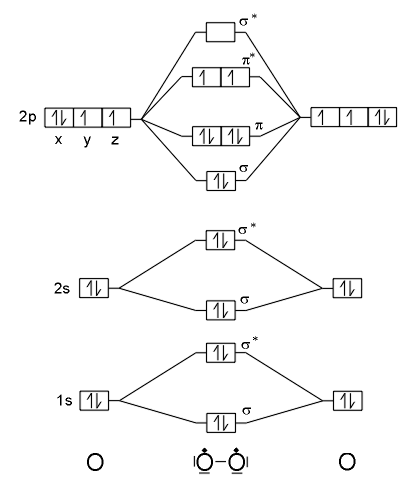
\includegraphics[width=0.5\textwidth]{_images/sauermo.png}
	
	\end{enumerate}
	
	%%%%%%%%%%%%%%%%%%%%%%%%%%%%%%%%%%%%%%%%%%%%%%%%%%%%%%%%
	
	\item Eine Verbindung, die aus 2.1\% \ce{H}, 29.8\% \ce{N} und 68,1\% \ce{O} besteht, hat
	ein Molekulargewicht von ca. 50 g/Mol. \\
	Wie lautet die Molek�lformel der Verbindung? \\
	Zeichnen sie die Lewis-Formel, wenn \ce{H} an \ce{O} gebunden ist. \\
	Wie ist die Struktur des Molek�ls? \\
	Wie ist die Hybridisierung der Orbitale am \ce{N}-Atom? \\
	Wie viele $\sigma$ - und $\pi$ -Bindungen gibt es in dem Molek�l?
	
	\begin{enumerate}
	
		\item 
		$M_{\ce{H}}	=1\frac{g}{Mol}$\\
		$M_{\ce{N}}	=14\frac{g}{Mol}$\\
		$M_{\ce{O}}	=16\frac{g}{Mol}$\\ 
		
		$\ce{H}:	\frac{2,1}{1}		=2,1Mol\%$\\
		$\ce{N}:	\frac{29,8}{14}		=2,13Mol\%$\\
		$\ce{O}:	\frac{68,1}{16}		=4,26Mol\%$\\ 
		
		$2,1 : 2,13 : 4,26 \Rightarrow 1:1:2 \Rightarrow \ce{HNO2}$
		
		\item
		
\includegraphics[width=0.2\textwidth]{_images/Lewis_Formel_Salpetrige_Saeure.png}
		
		\item
		Die Struktur ist trigonal eben.
		
		\item
		sp$^{2}$-Hybridisierung um N
		
		\item
		3 $\sigma$-Bindungen und 1 $\pi$-Bindung
		
	
	\end{enumerate}

	%%%%%%%%%%%%%%%%%%%%%%%%%%%%%%%%%%%%%%%%%%%%%%%%%%%%%%%%
	
\end{enumerate}




		%%%%%%%%%%%%%%%%%%%%%%%%%%%%%%%%%%%%%%%%%%%%%%%%%%%%%%%%%%%%%%%%%%%%%%%%%%
%%%%%%%%%%%%%%%%%%%%%%%%%%%%%%%%%%%%%%%%%%%%%%%%%%%%%%%%%%%%%%%%%%%%%%%%%%
\section*{GASE \& FL�SSIGKEITEN \& L�SUNGEN}
%%%%%%%%%%%%%%%%%%%%%%%%%%%%%%%%%%%%%%%%%%%%%%%%%%%%%%%%%%%%%%%%%%%%%%%%%%
%%%%%%%%%%%%%%%%%%%%%%%%%%%%%%%%%%%%%%%%%%%%%%%%%%%%%%%%%%%%%%%%%%%%%%%%%%

%%%%%%%%%%%%%%%%%%%%%%%%%%%%%%%%%%%%%
	\begin{karte}{
		Eine Gasmischung aus 6.00 g \ce{O2} und 9.00 g \ce{CH4} wird bei 0�C in einen Beh�lter (V = 100 mL) gegeben. \\
		Wie sind die Partialdr�cke f�r jedes Gas und wie ist der Gesamtdruck im Beh�lter in atm? \\
		$R = 0.0821  \frac{L\,atm}{Mol \,K}$
		}
		
		\begin{enumerate}
			
				\item 
				$M_{\ce{O2}}		=2\cdot16								=32\frac{g}{Mol}$\\
				$M_{\ce{CH4}}	=12+4\cdot1							=16\frac{g}{Mol}$\\
				$n_{\ce{O2}}		=\frac{6g}{32\frac{g}{Mol}}		=0,1875 Mol$\\
				$n_{\ce{CH4}}	=\frac{9g}{16\frac{g}{Mol}}		=0,5625 Mol$
				
				$\displaystyle pV=nRT \Rightarrow p=\frac{nRT}{V}$\\
						
				$\displaystyle P_{\ce{O2}}		=\frac{0,1875Mol\cdot0,0821\frac{L\,atm}{Mol \,K}\cdot273,15K}{0,1L}	=42atm$\\
				$\displaystyle P_{\ce{CH4}}	=\frac{0,5625Mol\cdot0,0821\frac{L\,atm}{Mol \,K}\cdot273,15K}{0,1L}	=126atm$
		
				$\displaystyle p_{ges} = \sum_{i=1}^k p_i$
				
				$P_{ges}					=42atm + 126atm					=168atm$
				
			\end{enumerate}
		
	\end{karte}
%%%%%%%%%%%%%%%%%%%%%%%%%%%%%%%%%%%%%

%%%%%%%%%%%%%%%%%%%%%%%%%%%%%%%%%%%%%
	\begin{karte}{
		Ammoniumnitrit zersetzt sich beim Erhitzen zu \ce{N2} Gas: \ce{NH4NO2 -> N_{2(g)} + 2H2O_{(l)}} 
		Wenn eine Probe in einem Reagenzglas zersetzt wird, werden 511 mL \ce{N2}-Gas �ber Wasser bei 26�C und 745 Torr Gesamtdruck aufgefangen. \\
		
		Wie viel Gramm Ammoniumnitrit wurden zersetzt? \\
		$R = 62,36 \frac{L\,torr}{Mol \,K}$
		}
		
		\begin{enumerate}
		
				\item 
				$M_{\ce{NH4NO2}}		=14+4\cdot1+14+2\cdot16	=64\frac{g}{Mol}$ 
				
				$\displaystyle n			=\frac{P\cdot V}{R\cdot T}		
									=\frac{745Torr \cdot 0,511 L}{62,36  \frac{L\,torr}{Mol \,K} \cdot (273,15+26)K}
									=0,02Mol$
				
				$m_{\ce{NH4NO2}}		=64\frac{g}{Mol} \cdot 0,02Mol		=1,28g$
				
			\end{enumerate}
		
	\end{karte}
%%%%%%%%%%%%%%%%%%%%%%%%%%%%%%%%%%%%%

%%%%%%%%%%%%%%%%%%%%%%%%%%%%%%%%%%%%%
	\begin{karte}{
		Cyclopropan, besteht aus 85.7 Massen\% \ce{C} und 14.3 Massen\% \ce{H}. 
			Wenn 1.56 g Cyclopropan ein Volumen von 1 L bei 0.984 atm und 50�C hat, 
			wie ist dann die Molek�lformel von Cyclopropan? \\
			W�rden Sie erwarten, dass Cyclopropan mehr oder weniger als Argon vom idealen Gasverhalten bei moderaten Dr�cken und Zimmertemperatur abweicht? \\
			Erkl�ren Sie! \\
			$R = 0.0821  \frac{L\,atm}{Mol \,K}$
		}
		
		\begin{enumerate}
			
				\item
				$M_{\ce{C}}	=12 \frac{g}{Mol}$ \\
				$M_{\ce{H}}	=1 \frac{g}{Mol}$ \\
			
			\end{enumerate}
		
	\end{karte}
%%%%%%%%%%%%%%%%%%%%%%%%%%%%%%%%%%%%%

%%%%%%%%%%%%%%%%%%%%%%%%%%%%%%%%%%%%%
	\begin{karte}{
		9.23 g einer Mischung von Magnesiumcarbonat und Calciumoxid wird mit einem �berschuss von Salzs�ure behandelt. Die resultierende Reaktion erzeugt 1.72 L Kohlendioxid bei 28�C und 743 Torr. \\
		Schreiben Sie ausgeglichene chemische Gleichungen f�r die Reaktionen, die zwischen der Salzs�ure und jedem Bestandteil der Mischung auftreten. \\
		Berechnen sie die Gesamtmolzahl von Kohlendioxid, die durch diese Reaktion gebildet wird. \\
		Unter der Annahme, dass die Reaktionen vollst�ndig ablaufen, berechnen sie die Massenprozent von Magnesiumcarbonat in der Mischung.\\
		(R = 62.36 L torr/Mol K)
		}
		
	\end{karte}
%%%%%%%%%%%%%%%%%%%%%%%%%%%%%%%%%%%%%

%%%%%%%%%%%%%%%%%%%%%%%%%%%%%%%%%%%%%
	\begin{karte}{
		Zeichnen und beschreiben Sie das Phasendiagramm von Wasser. \\
		Definieren Sie die beiden besonderen Punkte.
		}
		
	\end{karte}
%%%%%%%%%%%%%%%%%%%%%%%%%%%%%%%%%%%%%

%%%%%%%%%%%%%%%%%%%%%%%%%%%%%%%%%%%%%
	\begin{karte}{
		Welche Art von Anziehungskr�ften liegt zwischen Teilchen in \\
			a) molekularen Kristallen, \\
			b) kovalenten Kristallen, \\
			c) ionischen Kristallen und\\
			d) metallischen Kristallen vor?
		}
		
	\end{karte}
%%%%%%%%%%%%%%%%%%%%%%%%%%%%%%%%%%%%%

%%%%%%%%%%%%%%%%%%%%%%%%%%%%%%%%%%%%%
	\begin{karte}{
		Wie unterscheidet ein amorpher Festk�rper sich von einem kristallinen?\\
		Geben Sie je ein Beispiel f�r einen amorphen und einen kristallinen Festk�rper.
		}
		
	\end{karte}
%%%%%%%%%%%%%%%%%%%%%%%%%%%%%%%%%%%%%

%%%%%%%%%%%%%%%%%%%%%%%%%%%%%%%%%%%%%
	\begin{karte}{
		Glycerin ist ein wasserl�slicher Nichtelektrolyt mit einer Dichte
			von 1.26 g/mL bei 25�C. Berechnen sie den Dampfdruck einer
			L�sung, die durch Zugabe von 50 mL Glycerin zu 500 mL Wasser hergestellt
			wird. Der Dampfdruck von reinem Wasser bei 25�C betr�gt
			23.8 Torr.
		}
		
	\end{karte}
%%%%%%%%%%%%%%%%%%%%%%%%%%%%%%%%%%%%%

%%%%%%%%%%%%%%%%%%%%%%%%%%%%%%%%%%%%%
	\begin{karte}{
		Der Dampfdruck von reinem Wasser bei 110�C ist 1070 Torr.
			Eine L�sung aus Ethylenglykol und Wasser hat einen Dampfdruck von
			1.00 atm bei 110�C. Berechnen Sie den Molenbruch von Ethylenglykol.
		}
		
	\end{karte}
%%%%%%%%%%%%%%%%%%%%%%%%%%%%%%%%%%%%%

%%%%%%%%%%%%%%%%%%%%%%%%%%%%%%%%%%%%%
	\begin{karte}{
		Wenn 10.0 g \ce{Hg(NO3)2} in 1 kg Wasser aufgel�st wird, ist der
			Gefrierpunkt der L�sung -0.162 �C. Wenn 10.0 g \ce{HgCl2}
			in 1 kg Wasser gel�st werden, gefriert die L�sung bei -0.0685�C.
			Bestimmen sie anhand der dieser Daten, welches der st�rkere Elektrolyt
			ist und berechnen sie die Siedepunktserh�hung in beiden F�llen. ($K_{b\,\ce{H2O}}$
			= 0.51 �C/m)
		}
		
	\end{karte}
%%%%%%%%%%%%%%%%%%%%%%%%%%%%%%%%%%%%%



		%!TEX root = ../chemie.tex



\newpage

\chapter{CHEMISCHE KINETIK}
\begin{enumerate}

	%%%%%%%%%%%%%%%%%%%%%%%%%%%%%%%%%%%%%%%%%%%%%%%%%%%%%%%%
	
	\item F�r die Reaktion \ce{BF_{3(g)} + NH_{3(g)} -> F_{3}BNH_{3(g)}}
	wurden folgende Daten gemessen:\\
	 %
	\begin{tabular}{cccc}
	\hline 
	Versuch & \ce{BF_{3}} / $\frac{M}{L}$ & \ce{NH3} / $\frac{M}{L}$ & Anfangsreaktionsgeschw $\frac{M}{s}$ \tabularnewline
	\hline 
	\hline 
	1 & 0,25 & 0,25 & 0,1230\tabularnewline
	\hline 
	2 & 0,250 & 0,125 & 0,1065\tabularnewline
	\hline 
	3 & 0,200 & 0,100 & 0,0682\tabularnewline
	\hline 
	4 & 0,350 & 0,100 & 0,1193\tabularnewline
	\hline 
	5 & 0,175 & 0,100 & 0,0596\tabularnewline
	\hline 
	\end{tabular}\\
	Wie lautet das Geschwindigkeitsgestz f�r die Reaktion? Was ist die
	Gesamtordnung der Reaktion? Was ist der Wert f�r die Geschwindigkeitskonstante
	der Reaktion?
	
	\begin{enumerate}
	\item a
	\end{enumerate}
	\item Die Aktivierungsenergie einer bestimmten Reaktion ist $65.7kJ/Mol$.
	Wie viel schneller findet die Reaktion bei Die Zersetzung von Wasserstoffperoxid
	wird durch Jodidionen katalysiert. Man glaubt, dass die katalysierte
	Reaktion �ber einen zweistufigen Mechanismus abl�uft:
	\ce{H2O2 + I- -> H2O + IO-} (langsam) und \ce{IO- + H2O2 -> H2O + O2 + I-}
	(schnell) Schreiben Sie das Geschwindigkeitsgesetz f�r jede der
	Elementarreaktionen des Reaktionsmechanismuses an. 
	Schreiben Sie die chemische Gleichung f�r den Gesamtprozess. 
	Sagen Sie das Geschwindigkeitsgesetz f�r den Gesamtprozess vorher.
	
	\begin{enumerate}
	\item a
	\end{enumerate}
	\item Der erste Schritt eines Mechanismus bei der Reaktion von Brom ist:
	\ce{Br2 <-> 2Br} (schnell, im Gleichgewicht)\\
	Wie lautet der Ausdruck, der die Konzentration von \ce{Br} mit der von
	\ce{Br2} in Beziehung setzt?
	
	\begin{enumerate}
	\item a
	\end{enumerate}
	\item Viele metallische Katalysatoren, vor allem Edelmetallkatalysatoren,
	werden h�ufig als sehr d�nne Schichten auf einer Substanz mit hoher
	spezifischer Oberfl�che, wie Aluminiumoxid oder Siliziumoxid abgeschieden.
	Warum ist das ein effektives Verfahren zur Nutzung von Katalysatorstoffen?
	
	\begin{enumerate}
	\item a
	\end{enumerate}
	\end{enumerate}
	
	

%%%%%%%%%%%%%%%%%%%%%%%%%%%%%%%%%%%%%%%%%%%%%%%%%%%%%%%%





		%%%%%%%%%%%%%%%%%%%%%%%%%%%%%%%%%%%%%%%%%%%%%%%%%%%%%%%%%%%%%%%%%%%%%%%%%%
%%%%%%%%%%%%%%%%%%%%%%%%%%%%%%%%%%%%%%%%%%%%%%%%%%%%%%%%%%%%%%%%%%%%%%%%%%
\section*{CHEMISCHES GLEICHGEWICHT}
%%%%%%%%%%%%%%%%%%%%%%%%%%%%%%%%%%%%%%%%%%%%%%%%%%%%%%%%%%%%%%%%%%%%%%%%%%
%%%%%%%%%%%%%%%%%%%%%%%%%%%%%%%%%%%%%%%%%%%%%%%%%%%%%%%%%%%%%%%%%%%%%%%%%%

%%%%%%%%%%%%%%%%%%%%%%%%%%%%%%%%%%%%%
	\begin{karte}{
		
		Bestimmen Sie mit folgenden Informationen:\\
		\ce{HF <-> H+ + F-} $K_{c}=6.8 \cdot 10^{-4}$ und\\
		\ce{H2C2O4 <-> 2H+ + C2O4^{2-}} $K_{c}=3,8 \cdot 10^{-6}$\\
		die Gleichgewichtskonstante $K_{c}$ der Reaktion  \ce{2HF + C2O4^{2-} <-> 2F- + H2C2O4} (alle Reaktionspartner sind aquatisiert). Zeichnen sie eine plausible Lewis-Strukturformel von \ce{H2C2O4}.
		
		}
		
	\end{karte}
%%%%%%%%%%%%%%%%%%%%%%%%%%%%%%%%%%%%%

%%%%%%%%%%%%%%%%%%%%%%%%%%%%%%%%%%%%%
	\begin{karte}{
		
		Die Gleichgewichtskonstanten $K_{p}$ (bei 700�C) f�r die Reaktionen:\\
		\ce{H2 +I2 <-> 2HI} $K_{p}=54.0$,\\
		\ce{N2 + 3H2 <-> 2NH3} $K_{p}=1,04\cdot10^{-4}$ \\
		sind gegeben. Bestimmen Sie den Wert f�r $K_{p}$ f�r die Reaktion \ce{2NH3 + 3I2 <-> 6HI + N2} bei $700K$. (Alle Reaktionspartner sind im gasf�rmigen Zustand).
		
		}
		
	\end{karte}
%%%%%%%%%%%%%%%%%%%%%%%%%%%%%%%%%%%%%

%%%%%%%%%%%%%%%%%%%%%%%%%%%%%%%%%%%%%
	\begin{karte}{
		
		Schwefeltrioxid zersetzt sich bei hoher Temperatur in einem geschlossenen Beh�lter gem��: \ce{2SO3 <-> 2SO2 + O2} (Alle Reaktionspartner sind im gasf�rmigen Zustand). Ein Gef�� wird bei $1000K$ mit \ce{SO_{3}} bei einem Partialdruck von $0,500atm$ gef�llt. Im Gleichgewicht ist der Partialdruck von \ce{SO3} $0,200atm$. Berechnen sie den Wert f�r $K_{p}$ bei $1000K$.
		
		}
		
	\end{karte}
%%%%%%%%%%%%%%%%%%%%%%%%%%%%%%%%%%%%%

%%%%%%%%%%%%%%%%%%%%%%%%%%%%%%%%%%%%%
	\begin{karte}{
		
		Bei 1000 K ist der Wert f�r $K_{p}$ der Reaktion \\
		\ce{2SO3 <->2SO2 + O2}\\
		gleich $0,338$. Sagen sie vorher welche Reaktion abl�uft, wenn ein Gemisch mit den Anfangspartialdr�cken von \\
		$p_{\ce{SO3}}=0,16atm$; \\
		$p_{\ce{SO2}}=0.41atm$; \\
		$p_{\ce{O2}}=2.5atm$ betrachtet wird.
		
		}
		
	\end{karte}
%%%%%%%%%%%%%%%%%%%%%%%%%%%%%%%%%%%%%

%%%%%%%%%%%%%%%%%%%%%%%%%%%%%%%%%%%%%
	\begin{karte}{
		
		Schreiben sie den Gleichgewichtsausdruck f�r das Gleichgewicht: \ce{C_{(s)} + CO2_{(g)} <-> 2CO_{(g)}}.
		Die unten angef�hrte Tabelle zeigt die Molprozente von \ce{CO2} und \ce{CO} bei einem Gesamtdruck von 1 atm f�r mehrere Temperaturen.
		Berechnen sie den Wert von Kp bei jeder Temperatur. 
		Ist die Reaktion exotherm oder endotherm? 
		Begr�nden sie Ihre Antwort. (R = 0.0821 L atm/Mol K).

		\begin{tabular}{ccc}
			\hline 
			$Temperatur$ & $CO_{2}$ & $CO$ \tabularnewline
			$\celsius $ & $Mol\%$ & $Mol\%$ \tabularnewline
			\hline 
			\hline 
			$850$ & $6,23$ & $93,77$ \tabularnewline
			$950$ & $1,32$ & $98,68$ \tabularnewline
			$1050$ & $0,37$ & $99,63$ \tabularnewline
			\hline 
		\end{tabular}
		
		}
		
	\end{karte}
%%%%%%%%%%%%%%%%%%%%%%%%%%%%%%%%%%%%%

%%%%%%%%%%%%%%%%%%%%%%%%%%%%%%%%%%%%%
	\begin{karte}{
		
		F�r das Gleichgewicht \ce{PCl5 <-> PCl3 + Cl2} (Alle Reaktionspartner sind im gasf�rmigen Zustand) betr�gt Kp @ 500K 0.497. \\
		Eine Gasflasche wird bei einem Anfangsdruck von 1.66 atm gef�llt.\\
		Was sind die Gleichgewichtsdr�cke f�r die drei Gase bei dieser Temperatur?
		
		}
		
	\end{karte}
%%%%%%%%%%%%%%%%%%%%%%%%%%%%%%%%%%%%%


		%%%%%%%%%%%%%%%%%%%%%%%%%%%%%%%%%%%%%%%%%%%%%%%%%%%%%%%%%%%%%%%%%%%%%%%%%%
%%%%%%%%%%%%%%%%%%%%%%%%%%%%%%%%%%%%%%%%%%%%%%%%%%%%%%%%%%%%%%%%%%%%%%%%%%
\section*{S�URE-BASE GLEICHGEWICHTE}
%%%%%%%%%%%%%%%%%%%%%%%%%%%%%%%%%%%%%%%%%%%%%%%%%%%%%%%%%%%%%%%%%%%%%%%%%%
%%%%%%%%%%%%%%%%%%%%%%%%%%%%%%%%%%%%%%%%%%%%%%%%%%%%%%%%%%%%%%%%%%%%%%%%%%


%%%%%%%%%%%%%%%%%%%%%%%%%%%%%%%%%%%%%
	\begin{karte}{
		
		Der pH-Wert von 0.62 g Niacin in 250 mL Wasser betr�gt bei 25�C 3.26. Wie gro� ist die S�urekonstante $K_{s}$ und wie viel Prozent Nicatin sind unter diesen Bedingungen dissoziiert?\\
		
\includegraphics{_images/1.pdf}
		
		}
		
	\end{karte}
%%%%%%%%%%%%%%%%%%%%%%%%%%%%%%%%%%%%%

%%%%%%%%%%%%%%%%%%%%%%%%%%%%%%%%%%%%%
	\begin{karte}{
		
	Berechnen sie den Prozentsatz an dissoziierten \ce{HF} Molek�len in w�ssrigen \ce{HF}-L�sungen von 0.10 Mol/L und von 0.01 Mol/L. $K_{S}=6,8\cdot10^{-4}$
		
		}
		
	\end{karte}
%%%%%%%%%%%%%%%%%%%%%%%%%%%%%%%%%%%%%

%%%%%%%%%%%%%%%%%%%%%%%%%%%%%%%%%%%%%
	\begin{karte}{
		
		Berechnen sie den pH-Wert einer Oxals�urel�sung \ce{(COOH)_{2}} mit einer Konzentration von 0.020 Mol/L bei 25�C. $K{}_{S1}=5,9\cdot10^{-2}$;
		$K_{S2}=6,4\cdot10^{-5}$. Bestimmen Sie die Konzentration des Oxalations \ce{(COO)_{2}^{2-}} in der L�sung.
		
		}
		
	\end{karte}
%%%%%%%%%%%%%%%%%%%%%%%%%%%%%%%%%%%%%

%%%%%%%%%%%%%%%%%%%%%%%%%%%%%%%%%%%%%
	\begin{karte}{
		
		Phosphorige S�ure \ce{(H_{3}PO_{3})} besitzt die rechts gezeigte Lewis Strukturformel: Erkl�ren Sie, warum \ce{H3PO3} zweibasig und nicht dreibasig ist. Es werden 25 mL \ce{H_{3}PO_{3}} mit einer 0.102 Mol/L \ce{NaOH}-L�sung titriert. Dabei werden 23.3 mL dieser L�sung ben�tigt um die \ce{H3PO3} zu neutralisieren. Welche Molarit�t hat die \ce{H3PO3}-L�sung? Der pH-Wert der L�sung betr�gt 1.59. 
		
		Berechnen sie $K_{S1}$ und den Dissoziationsgrad unter der Annahme, dass $K_{S2}$ vernachl�ssigt werden kann.\\
		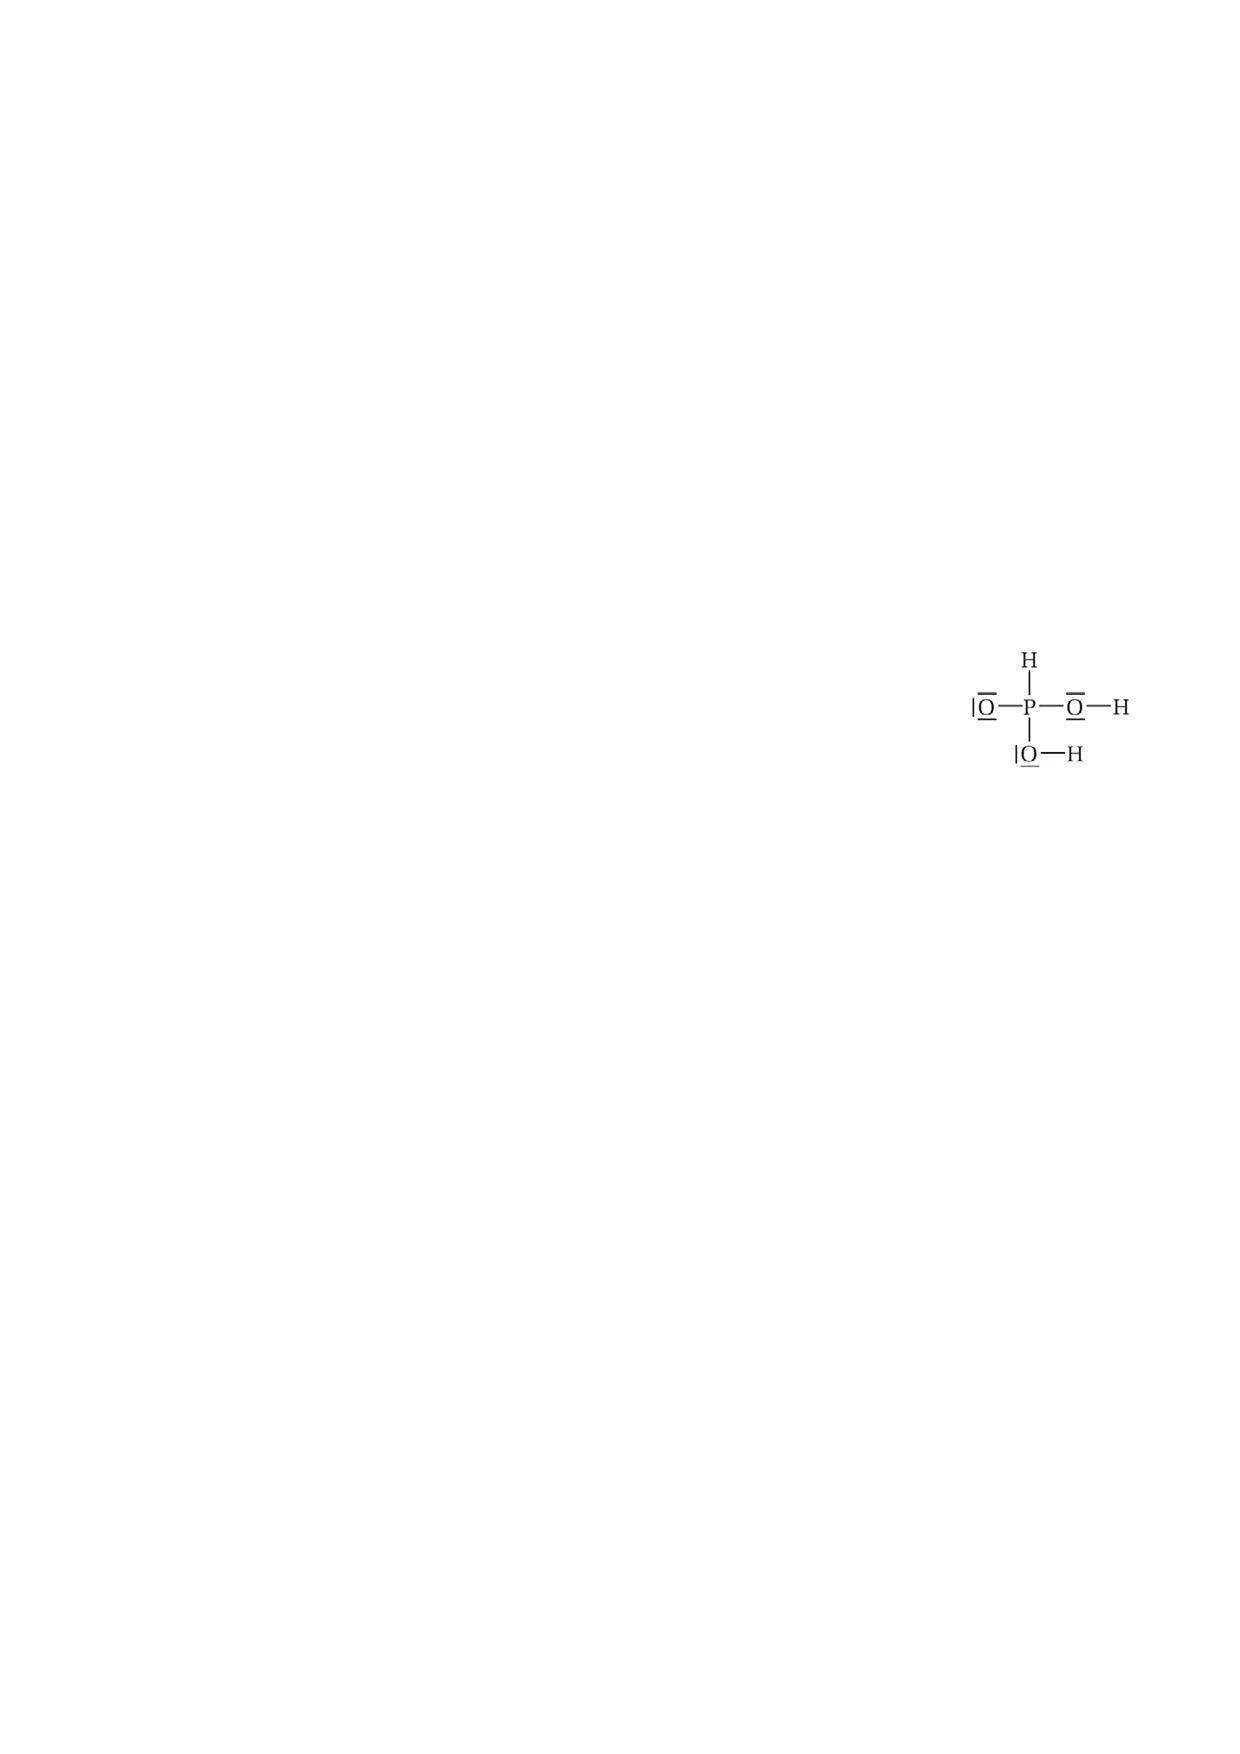
\includegraphics[width=0.3\textwidth, angle=0]{_images/2.pdf}
		
		
		}
		
	\end{karte}
%%%%%%%%%%%%%%%%%%%%%%%%%%%%%%%%%%%%%

%%%%%%%%%%%%%%%%%%%%%%%%%%%%%%%%%%%%%
	\begin{karte}{
		
		Berechnen Sie die Konzentration des Fluoridions und den pH-Wert einer L�sung mit 0.20 Mol/L \ce{HF} und 0.10 Mol/L \ce{HCl}. $(K_{S\, HF}=6,8\cdot10^{-4})$
		
		}
		
	\end{karte}
%%%%%%%%%%%%%%%%%%%%%%%%%%%%%%%%%%%%%

%%%%%%%%%%%%%%%%%%%%%%%%%%%%%%%%%%%%%
	\begin{karte}{
		
		Welchen pH-Wert hat eine L�sung aus 0.30 Mol Essigs�ure und 0.30 Mol Natriumacetat, zu denen soviel Wasser gegeben wird, dass 1.0 L L�sung entsteht? $(K_{S\, Essigs\ddot{a}ure}=1,8\cdot10^{-5})$
		
		}
		
	\end{karte}
%%%%%%%%%%%%%%%%%%%%%%%%%%%%%%%%%%%%%

%%%%%%%%%%%%%%%%%%%%%%%%%%%%%%%%%%%%%
	\begin{karte}{
		
		Welchen pH-Wert hat ein Puffer mit 0.12 Mol/L Benzoes�ure und 0.20 Mol/L Natriumbenzoat? $(K_{S\, Benzoes\ddot{a}ure}=6,3\cdot10^{-5})$
		
		}
		
	\end{karte}
%%%%%%%%%%%%%%%%%%%%%%%%%%%%%%%%%%%%%

%%%%%%%%%%%%%%%%%%%%%%%%%%%%%%%%%%%%%
	\begin{karte}{
		
		Berechnen sie den pH-Wert. Der sich einstellt, wenn 45 mL einer 0.100 Mol/L \ce{NaOH}-L�sung zu einer 25 mL einer 0.100 Mol/L Essigs�urel�sung gegeben werden. $(K_{S\, Essigs\ddot{a}ure}=1,8\cdot10^{-5})$
		
		}
		
	\end{karte}
%%%%%%%%%%%%%%%%%%%%%%%%%%%%%%%%%%%%%

%%%%%%%%%%%%%%%%%%%%%%%%%%%%%%%%%%%%%
	\begin{karte}{
		
		Der Wert von $K_{L}$ von \ce{CaF_{2}} ist bei 25�C gleich $3.9\cdot10^{-11}Mol^{3}/L^{3}$. Berechnen Sie die L�slichkeit von \ce{CaF2} in Gramm/Liter.
		
		}
		
	\end{karte}
%%%%%%%%%%%%%%%%%%%%%%%%%%%%%%%%%%%%%

%%%%%%%%%%%%%%%%%%%%%%%%%%%%%%%%%%%%%
	\begin{karte}{
		
		Bildet sich beim Mischen von $0.1L$ $8,0\cdot10^{-3}Mol/L$ \ce{Pb(NO3)2} und $0.4L$ $5,0\cdot10^{-3}$ $Mol/L$ \ce{Na2SO4} ein Niederschlag?
		$(K_{L_{8\ce{PbSO4}}}=6,3\cdot10^{-7}Mol^{2}/L^{2})$ 
		
		}
		
	\end{karte}
%%%%%%%%%%%%%%%%%%%%%%%%%%%%%%%%%%%%%


		%%%%%%%%%%%%%%%%%%%%%%%%%%%%%%%%%%%%%%%%%%%%%%%%%%%%%%%%%%%%%%%%%%%%%%%%%%
%%%%%%%%%%%%%%%%%%%%%%%%%%%%%%%%%%%%%%%%%%%%%%%%%%%%%%%%%%%%%%%%%%%%%%%%%%
\section*{THERMODYNAMIK II}
%%%%%%%%%%%%%%%%%%%%%%%%%%%%%%%%%%%%%%%%%%%%%%%%%%%%%%%%%%%%%%%%%%%%%%%%%%
%%%%%%%%%%%%%%%%%%%%%%%%%%%%%%%%%%%%%%%%%%%%%%%%%%%%%%%%%%%%%%%%%%%%%%%%%%

%%%%%%%%%%%%%%%%%%%%%%%%%%%%%%%%%%%%%
	\begin{karte}{
		
		Sagen sie voraus, ob $\Delta$S f�r folgende Prozesse positiv oder negativ ist, wobei wir davon ausgehen, dass alle bei konstanter Temperatur ablaufen:\\
		(a) \ce{H2O_{(g)} -> H2O_{(l)}}\\
		(b) \ce{Ag_{(aq)}^{+} + Cl_{(aq)}^{-} -> AgCl_{(s)}}\\
		(c) \ce{4Fe_{(s)} + 3O2_{(g)} -> 2Fe2O3_{(s)}}\\
		(d) \ce{N2_{(g)} + O2_{(g)} -> 2NO_{(g)}}
		
		}
		
	\end{karte}
%%%%%%%%%%%%%%%%%%%%%%%%%%%%%%%%%%%%%

%%%%%%%%%%%%%%%%%%%%%%%%%%%%%%%%%%%%%
	\begin{karte}{
		
		(a) Was ist das Besondere an einem reversiblen Prozess? \\
		(b) Gehen Sie davon aus, dass ein reversibler Prozess umgekehrt wird, und das System in seinen Ausgangszustand zur�ckversetzt wird. Was l�sst sich �ber die Umgebung nach der Umkehrung des Prozesses aussagen? \\
		(c) Unter welchen Umst�nden handelt es sich beim Verdampfen von Wasser zu Dampf um einen reversiblen Prozess?
		
		}
		
	\end{karte}
%%%%%%%%%%%%%%%%%%%%%%%%%%%%%%%%%%%%%

%%%%%%%%%%%%%%%%%%%%%%%%%%%%%%%%%%%%%
	\begin{karte}{
		
		Vervollst�ndigen Sie folgende Redoxgleichung: \\
		\ce{MnO- + Fe2+ + H+ -> MnO2 + Fe^{3+} + H2O}
		
		}
		
	\end{karte}
%%%%%%%%%%%%%%%%%%%%%%%%%%%%%%%%%%%%%

%%%%%%%%%%%%%%%%%%%%%%%%%%%%%%%%%%%%%
	\begin{karte}{
	
		Vervollst�ndigen Sie folgende Redoxgleichung:\\
		\ce{MnO4- + Mn^{2+} + H+ -> MnO2 + H2O}
		
		}
		
	\end{karte}
%%%%%%%%%%%%%%%%%%%%%%%%%%%%%%%%%%%%%

%%%%%%%%%%%%%%%%%%%%%%%%%%%%%%%%%%%%%
	\begin{karte}{
		
		Vervollst�ndigen Sie folgende Redoxgleichung: \\
		\ce{Cr2O7^{2-} + CH3OH + H+ -> Cr^{3+} + CO2 + H2O}
		
		}
		
	\end{karte}
%%%%%%%%%%%%%%%%%%%%%%%%%%%%%%%%%%%%%

%%%%%%%%%%%%%%%%%%%%%%%%%%%%%%%%%%%%%
	\begin{karte}{
		
		Beschreiben sie mit Hilfe einer Skizze den Aufbau einer Alkalibatterie und Formulieren Sie die Anoden und Kathodenreaktion.
		
		}
		
	\end{karte}
%%%%%%%%%%%%%%%%%%%%%%%%%%%%%%%%%%%%%

%%%%%%%%%%%%%%%%%%%%%%%%%%%%%%%%%%%%%
	\begin{karte}{
		
		Beschreiben sie mit Hilfe einer Skizze die Korrosion von Eisen und formulieren Sie die Anoden und Kathodenreaktion, sowie die Gesamtreaktion.
		
		}
		
	\end{karte}
%%%%%%%%%%%%%%%%%%%%%%%%%%%%%%%%%%%%%



		%!TEX root = ../chemie.tex




\newpage

\chapter{STOFFCHEMIE}

\begin{enumerate}

	%%%%%%%%%%%%%%%%%%%%%%%%%%%%%%%%%%%%%%%%%%%%%%%%%%%%%%%%
	
	\item Beschreiben sie Eigenschaften und Verwendung von Schwefel und Selen.
	
	\begin{enumerate}
		\item a
	\end{enumerate}

	%%%%%%%%%%%%%%%%%%%%%%%%%%%%%%%%%%%%%%%%%%%%%%%%%%%%%%%%
	\item Beschreiben sie die Herstellung und Verwendung von Stickstoff.
	
	\begin{enumerate}
		\item a
	\end{enumerate}

	%%%%%%%%%%%%%%%%%%%%%%%%%%%%%%%%%%%%%%%%%%%%%%%%%%%%%%%%

	\item Beschreiben sie Vorkommen und Herstellung von Silizium.
	
	\begin{enumerate}
		\item a
	\end{enumerate}

	%%%%%%%%%%%%%%%%%%%%%%%%%%%%%%%%%%%%%%%%%%%%%%%%%%%%%%%%

	\item Beschreiben sie die Herstellung von Stahl. Zeichnen sie drei Isomere
	der Summenformel \ce{C5H12} und geben sie einen chemischen Namen f�r jede
	
	\begin{enumerate}
		\item a
	\end{enumerate}

	%%%%%%%%%%%%%%%%%%%%%%%%%%%%%%%%%%%%%%%%%%%%%%%%%%%%%%%%

	\item Zeichnen sie die Strukturformeln des cis- und des trans-Isomers von
	3- Penten-1-ol. Kann bei Cyclopenten eine cis-trans Isomerie vorliegen?
	Erkl�ren sie ihre Antwort.
	
	\begin{enumerate}
		\item a
	\end{enumerate}

	%%%%%%%%%%%%%%%%%%%%%%%%%%%%%%%%%%%%%%%%%%%%%%%%%%%%%%%%

	\item Beschreiben Sie die sechs Kohlenwasserstofffraktionen der Erd�ldestillation,
	deren Siedepunktsbereiche und deren Verwendung.
	
	\begin{enumerate}
		\item a
	\end{enumerate}

	%%%%%%%%%%%%%%%%%%%%%%%%%%%%%%%%%%%%%%%%%%%%%%%%%%%%%%%%

	\item Beschreiben Sie die molekulare Grundlage unserer Sehf�higkeit.
	
	\begin{enumerate}
		\item a
	\end{enumerate}

	%%%%%%%%%%%%%%%%%%%%%%%%%%%%%%%%%%%%%%%%%%%%%%%%%%%%%%%%

	\item Definieren Sie Chiralit�t und zeichnen Sie ein beliebiges chirales
	Molek�l.
	
	\begin{enumerate}
		\item a
	\end{enumerate}

	%%%%%%%%%%%%%%%%%%%%%%%%%%%%%%%%%%%%%%%%%%%%%%%%%%%%%%%%

	\item Zeichnen Sie drei beliebige nat�rliche Aminos�uren und beschreiben
	Sie die Natur der Peptidbindung.
	
	\begin{enumerate}
		\item a
	\end{enumerate}

	%%%%%%%%%%%%%%%%%%%%%%%%%%%%%%%%%%%%%%%%%%%%%%%%%%%%%%%%

	\item Zeichnen Sie die Wiederholeinheit von Polyethylen, Polystyrol und
	Nylon 6,6. Geben sie je zwei Anwendungsgebiete dieser Kunststoffe
	an.

	\begin{enumerate}
		\item a
	\end{enumerate}
		
	%%%%%%%%%%%%%%%%%%%%%%%%%%%%%%%%%%%%%%%%%%%%%%%%%%%%%%%%

\end{enumerate}



%%%%%%%%%%%%%%%%%%%%%%%%%%%%%%%%%%%%%%%%%%%%%%%%%%%%%%%%



		%%%%%%%%%%%%%%%%%%%%%%%%%%%%%%%%%%%%%%%%%%%%%%%%%%%%%%%%%%%%%%%%%%%%%%%%%%
%%%%%%%%%%%%%%%%%%%%%%%%%%%%%%%%%%%%%%%%%%%%%%%%%%%%%%%%%%%%%%%%%%%%%%%%%%
\section*{ALLGEMEINE FRAGEN}
%%%%%%%%%%%%%%%%%%%%%%%%%%%%%%%%%%%%%%%%%%%%%%%%%%%%%%%%%%%%%%%%%%%%%%%%%%
%%%%%%%%%%%%%%%%%%%%%%%%%%%%%%%%%%%%%%%%%%%%%%%%%%%%%%%%%%%%%%%%%%%%%%%%%%

%%%%%%%%%%%%%%%%%%%%%%%%%%%%%%%%%%%%%
\begin{karte}{
	%Frage
	Wie ist das Periodensystem aufgebaut und welche Informationen kann man daraus ablesen.

	}
	%Antwort
	Antwort

\end{karte}
%%%%%%%%%%%%%%%%%%%%%%%%%%%%%%%%%%%%%

%%%%%%%%%%%%%%%%%%%%%%%%%%%%%%%%%%%%%
\begin{karte}{
	
	Welche chemischen Bindungen kennen Sie? Geben Sie zu jeder ein Beispiel und erkl�ren Sie.
	
	}
	
	Antwort
	
\end{karte}
%%%%%%%%%%%%%%%%%%%%%%%%%%%%%%%%%%%%%

%%%%%%%%%%%%%%%%%%%%%%%%%%%%%%%%%%%%%
\begin{karte}{
	
	Wie h�ngen die 1. Ionisierungsenergie und Elektronenaffinit�t mit der Lage im Periodensystem zusammen?
	
	}
	
	Antwort
	
\end{karte}
%%%%%%%%%%%%%%%%%%%%%%%%%%%%%%%%%%%%%

%%%%%%%%%%%%%%%%%%%%%%%%%%%%%%%%%%%%%
\begin{karte}{
	
	Welche Arten der chemischen Formelschreibweise kennen Sie? Geben sie jeweils ein Beispiel an.
	
	}
	
	Antwort
	
\end{karte}
%%%%%%%%%%%%%%%%%%%%%%%%%%%%%%%%%%%%%

%%%%%%%%%%%%%%%%%%%%%%%%%%%%%%%%%%%%%
\begin{karte}{
	
	Unter welchen Bedingungen kommt es zu einer sigma- und unter welchen Bedingungen zu einer pi \textendash{} Bindung? Erkl�ren Sie anhand eines Beispiels.
	
	}
	
	Antwort
	
\end{karte}
%%%%%%%%%%%%%%%%%%%%%%%%%%%%%%%%%%%%%

%%%%%%%%%%%%%%%%%%%%%%%%%%%%%%%%%%%%%
\begin{karte}{
	
	Welche Gasgesetze kennen Sie und welche Gr��en bringen sie in Zusammenhang?
	
	}
	
	Antwort
	
\end{karte}
%%%%%%%%%%%%%%%%%%%%%%%%%%%%%%%%%%%%%

%%%%%%%%%%%%%%%%%%%%%%%%%%%%%%%%%%%%%
\begin{karte}{
	
	Nennen Sie die wichtigsten Kennzeichen von Polymeren. Nennen Sie drei und geben ihre Verwendung an.
	
	}
	
	Antwort
	
\end{karte}
%%%%%%%%%%%%%%%%%%%%%%%%%%%%%%%%%%%%%

%%%%%%%%%%%%%%%%%%%%%%%%%%%%%%%%%%%%%
\begin{karte}{
	
	Was bedeutet L�slichkeit und wovon h�ngt die L�slichkeit eines Stoffes ab?
	
	}
	
	Antwort
	
\end{karte}
%%%%%%%%%%%%%%%%%%%%%%%%%%%%%%%%%%%%%}

%%%%%%%%%%%%%%%%%%%%%%%%%%%%%%%%%%%%%
\begin{karte}{
	
	Welche Konzentrationsangaben kennen Sie und wie sind sie jeweils definiert?
	
	}
	
	Antwort
	
\end{karte}
%%%%%%%%%%%%%%%%%%%%%%%%%%%%%%%%%%%%%

%%%%%%%%%%%%%%%%%%%%%%%%%%%%%%%%%%%%%
\begin{karte}{
	
	Welche kolligativen Eigenschaften kennen Sie und was wissen Sie dar�ber?
	
	}
	
	Antwort
	
\end{karte}
%%%%%%%%%%%%%%%%%%%%%%%%%%%%%%%%%%%%%

%%%%%%%%%%%%%%%%%%%%%%%%%%%%%%%%%%%%%
\begin{karte}{
	
	Wovon ist die Reaktionsgeschwindigkeit abh�ngig und was bedeutet Katalyse?
	
	}
	
	Antwort
	
\end{karte}
%%%%%%%%%%%%%%%%%%%%%%%%%%%%%%%%%%%%%

%%%%%%%%%%%%%%%%%%%%%%%%%%%%%%%%%%%%%
\begin{karte}{
	
	Erkl�ren Sie den Inhalt der 3 Haupts�tze der Thermodynamik.
	
	}
	
	Antwort
	
\end{karte}
%%%%%%%%%%%%%%%%%%%%%%%%%%%%%%%%%%%%%

%%%%%%%%%%%%%%%%%%%%%%%%%%%%%%%%%%%%%
\begin{karte}{
	
	Erkl�ren Sie die Begriffe Aminos�uren, Peptid und Protein.
	
	}
	
	Antwort
	
\end{karte}
%%%%%%%%%%%%%%%%%%%%%%%%%%%%%%%%%%%%%

%%%%%%%%%%%%%%%%%%%%%%%%%%%%%%%%%%%%%
\begin{karte}{
	
	Erkl�ren Sie die Begriffe Kohlenhydrat, Monosaccharid, Disaccharid und Polysaccharid und geben sie jeweils ein Beipiel an.
	
	}
	
	Antwort
	
\end{karte}
%%%%%%%%%%%%%%%%%%%%%%%%%%%%%%%%%%%%%

%%%%%%%%%%%%%%%%%%%%%%%%%%%%%%%%%%%%%
\begin{karte}{
	
	Erkl�ren Sie die Begriffe DNA, RNA, Nukleins�ure, Nukleotid.
	
	}
	
	Antwort
	
\end{karte}
%%%%%%%%%%%%%%%%%%%%%%%%%%%%%%%%%%%%%










\end{document}			%% Dokument ENDE %%%%%%%%%%%%%%%%%%%%%%%%%%%%%%%%%%%%%%%%%%%%%%%%%%%%%%%%%%







